\chapter{相变}
    \section{相变概念}
        关于相变,有一些最为基础的概念,
        \begin{enumerate}
            \item 相\index{相}:成分相同、结构相同,有界面同其他部分分隔的物质均匀组成部分;
            \item 相变\index{相变}:当外界条件(如温度、压力等)连续变化时,物质自身发生突变的现象。或物相的某个(阶)热力学势跃变,伴随物相的某个(些)要素跃变;
            \item 固态相变\index{固态相变}:固体材料的结构在温度、压力、成分改变时所发生的转变。
        \end{enumerate}

        在分类上,有很多种分类方法,比如从动力学上,或者是从热力学上分类
            \subsection{动力学相变分类}
                相变分为两类:扩散性和无扩散型,如\autoref{金属及合金中的一级相变}所示。
                无扩散型相变\index{无扩散型相变}较为简单,分为连续型相变\index{连续型相变},比如$\omega$相比\index{$\omega$相变},和形核长大型相变\index{形核长大型相变},比如马氏体相变\index{马氏体相变}。

                而扩散性相变\index{扩散性相变}则相对复杂,也分为连续型相变\index{连续型相变}和形核长大型相变\index{形核长大型相变},更为具体的分类将在后面的章节进行讲解,在这里不再进行过多叙述。
                \begin{figure}[ht]
                    \centering
                    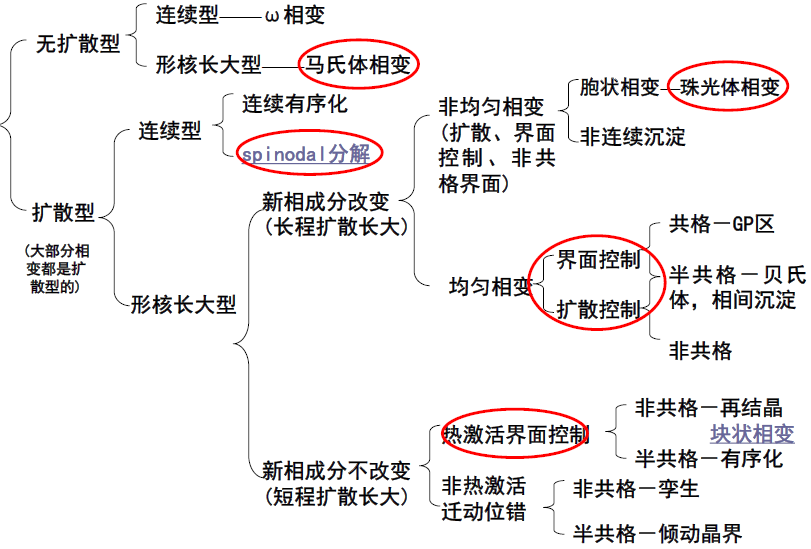
\includegraphics[width=0.7\textwidth]{fig/金属及合金中的一级相变.png}
                    \caption{金属及合金中的一级相变。}
                    \label{金属及合金中的一级相变}
                \end{figure}
            \subsection{热力学的相变分类}
                在热力学的分类比较简单,分为一级相变\index{一级相变}和二级相变\index{二级相变}。
                一级相变是指化学位相等,但是化学位的一阶导数不等,也就是熵不等或者是体积不等,
                \begin{align}
                    \mu_1&=\mu_2,\\
                    \left(  \frac{\partial\mu_1}{\partial T} \right)_p=-S_1&\neq-S_2= \left(  \frac{\partial\mu_2}{\partial T} \right)_p\label{等压一级相变},\\
                    \left(  \frac{\partial\mu_1}{\partial p} \right)_T=V_1&\neq V_2= \left(  \frac{\partial\mu_2}{\partial p} \right)_T\label{等温一级相变}.
                \end{align}
                在一级相变中伴有能量变化,或者吸热或者放热,或者体积发生变化。比如晶体的熔化、升华、液体的凝固、汽化、气体的凝聚以及晶体中大多数晶型转变都属于一级相变,这是最普遍的相变类型。

                二级相变是指化学位的二阶导数发生突变,而化学位和一阶导数不发生突变,
                \begin{align}
                    -\frac{C_p}{T}=\left(  \frac{ \partial^2\mu_1  }{\partial T^2} \right)_p&\neq\left(  \frac{ \partial^2\mu_2  }{\partial T^2} \right)_p,\\
                    kV=\left(  \frac{ \partial^2\mu_1  }{\partial p^2} \right)_T&\neq\left(  \frac{ \partial^2\mu_2  }{\partial p^2} \right)_T,\\
                    \alpha V=\frac{\partial^2\mu_1}{\partial T\partial p}&\neq\frac{\partial^2\mu_2}{\partial T\partial p}.
                \end{align}
                其中$C_p$为等压比热\index{等压比热},$k$为等温等压系数\index{等温等压系数},$\alpha$为等压膨胀系数\index{等压膨胀系数}\footnote{熔化、马氏体转变属一级相变,有序化可能是一级也
                可能是二级相变。}。
                在二级相变中,两相的化学势、熵和体积相等,但热容、膨胀系数和压缩系数不相等,即无相变潜热,无体积的突变,只有热容、
                膨胀系数和压缩系数的不连续变化,
                \begin{align*}
                    \Delta C_p\neq 0,\\
                    \Delta\beta\neq 0,\\
                    \Delta\alpha\neq0.\\
                \end{align*}
                一般合金的有序-无序转变、铁磁-顺磁转变、超导转变等属于二级相变。大多数便随某种物理性能的变化。
            \subsection{固溶体自由能的计算}
                纯组元的自由能和温度的关系可以写作
                \begin{equation}
                    G(T)=H(T)-TS(T),
                \end{equation}
                而两相混合的自由能,在理想条件下可以由两相的自由能叠加得到。

                假设在体系中存在两种相$\alpha$和$\beta$,均是由A、B两种原子构成,假设A原子的成分为$x\mathrm{at.}\%$,在$\alpha$相中,A的原子百分比为$x_1$,在$\beta$中的原子百分比为$x_2$
                而$\alpha$相和$\beta$的占比分别为$N_1$和$N_2$,两者的自由能分别为$G_1$和$G_2$,混合后的自由能为
                \begin{equation}
                    G=N_1G_1+N_2G_2,
                \end{equation}
                利用成分关系,可以变为
                \begin{equation}
                    G=G_1+\frac{x-x_1}{x_2-x_1}(G_2-G_1),
                \end{equation}
                所以$G_1$,$G$,$G_2$处于同一直线,并且服从杠杆定律。

                但是在混合过程存在其他作用,导致混合后的自由能不等于理想情况下的自由能。这里假设实际的自由能为
                \begin{equation}
                    G(x)=G^0+\Delta G^m,
                \end{equation}
                其中
                \begin{equation}
                    G^0=x_AG_A^0+x_BG_B^0,
                \end{equation}
                其中,$x_A$为$A$原子的原子百分比,$x_B$为$B$原子的原子百分比,而要计算$\Delta G^m$,需要先计算混合过程中的焓\index{焓}和熵\index{熵}的变化量。
                \subsubsection{混合过程中熵的改变量}
                    固态下的系统的熵主要由混合熵\index{熵!混合熵}(决定于原子可能排列的方式)和振动熵\index{熵!振动熵}(决定于温度和缺陷)组成,
                    混合熵的变化为
                    \begin{equation}
                        \Delta S^m=S_{AB}-(x_AS_A+x_BS_B),
                    \end{equation}
                    根据混合熵的定义
                    \begin{equation}
                        S=k\ln{\Omega},
                    \end{equation}
                    其中$k$为玻尔兹曼常数,$\Omega$为微观状态数,假设$A$的原子数为$N_A$,$B$的原子数为$N_B$,混合熵的变化为
                    \begin{equation}
                        \begin{split}
                        \Delta S^m&=S_{AB}-(x_AS_A+x_BS_B)\\
                        &=k\ln{\frac{N!}{N_A!(N-N_A)!}}-x_Ak \ln \left(C_{N_{A}}^{N_{A}}\right)  -x_Bk \ln \left(C_{N_{B}}^{N_{B}}\right)\\
                        &=k\ln{\frac{N!}{N_A!N_B!}}\\
                        &=k\left( \ln{N!}-\ln{N_A!}-\ln{N_B!} \right).                
                        \end{split}                                      
                    \end{equation}
                    根据Stirling公式,
                    \begin{equation}
                        \Delta S^m=-R(x_A\ln{x_A}+x_B\ln{x_B}),
                    \end{equation}
                    其中$R=kN$。
                \subsubsection{混合过程中焓的改变量}
                    接下来计算混合过程中焓的变化,利用溶液的准化学模型\index{准化学模型},假设
                    \begin{enumerate}
                        \item $A$,$B$两组元尺寸接近,排列无序;
                        \item 混合过程中体积基本不变,即$\Delta V=0$;
                        \item 原子只与最近邻的原子之间存在相互作用,即只计算最近邻原子之间的结合能。
                    \end{enumerate}
                    假设两个近邻原子之间额定结合能分别为$u_{AA}$、$u_{AB}$和$u_{BB}$,固溶体和组元的配位数均为$Z$。在恒压情况下,焓的改变仅与结合能的改变有关,
                    所以
                    \begin{align}
                        \text{混合前,}&u_{1}=\frac{1}{2} N_{A} Z u_{A A}+\frac{1}{2} N_{B} Z u_{B B},\\
                        \text{混合后,}&u_{2}=\frac{1}{2} N_{A} Z \frac{N_{A}}{N} u_{A A}+\frac{1}{2} N_{B} Z \frac{N_{B}}{N} u_{B B}+N_{A} Z \frac{N_{B}}{N} u_{A B}.
                    \end{align}
                    所以焓的变化量为
                    \begin{equation}
                        \Delta u^m=Z N\left(u_{A B}-\frac{u_{A A}+u_{B B}}{2}\right) x_{A} x_{B},
                    \end{equation}
                    令$\alpha'=ZN\left( u_{AB}-\frac{u_{AA}+u_{BB}}{2} \right)$,焓变可以写作
                    \begin{equation}
                        \Delta H^m=\alpha'x_Ax_B.
                    \end{equation}
            \subsection{混合过程的自由能改变量以及成分与自由能关系}
                所以混合过程中自由能随成分和温度变化的关系为
                \begin{equation}
                    G(x)=G_{A}^{0} x_{A}+G_{B}^{0} x_{B}+\alpha^{\prime} x_{A} x_{B}+R T\left(x_{A} \ln x_{A}+x_{B} \ln x_{B}\right)\label{混合过程的自由能曲线}.
                \end{equation}
                下面将对于这一曲线进行讨论。

                混合前的自由能为$G_{A}^{0} x_{A}+G_{B}^{0} x_{B}$为一条直线,而熵的改变量则由于成分百分比均小于1而小于0,但是$\alpha^{\prime}$,也就是原子结合能的改变量不是能够确定的事,需要分情况讨论。
                在此之前,先进一步确定曲线与成分的关系,
                \begin{align}
                    \frac{\partial G}{\partial x_{B}}&=-G_{A}^{0}+G_{B}^{0}+\alpha^{\prime}\left(x_{A}-x_{B}\right)+R T\left(\ln x_{B}-\ln x_{A}\right),\\
                    \frac{\partial^{2} G}{\partial x_{B}^{2}}&=-2 \alpha^{\prime}+R T\left(\frac{1}{x_{A}}+\frac{1}{x_{B}}\right).
                \end{align}
                由此可见,曲线中唯有成分也就是结合能的变化不能确定,下面将针对结合能变化的三种情况进行讨论。

                当原子结合能不发生改变时,也就是$\alpha^{\prime}=0$时,此时体系符合理想溶液模型,自由能的二阶导数
                \begin{equation}
                    \frac{\partial^{2} G}{\partial x_{B}^{2}}=R T\left(\frac{1}{x_{A}}+\frac{1}{x_{B}}\right)>0,
                \end{equation}
                $G(x)$为下垂线,及曲线的凹向朝上,如\autoref{混合时结合能不变的自由能曲线}所示。
                \begin{figure}[ht]
    \centering
    %\begin{subfigure}[0.3\textwidth]
    \subfigure[混合时结合能不变的自由能曲线]
    {
        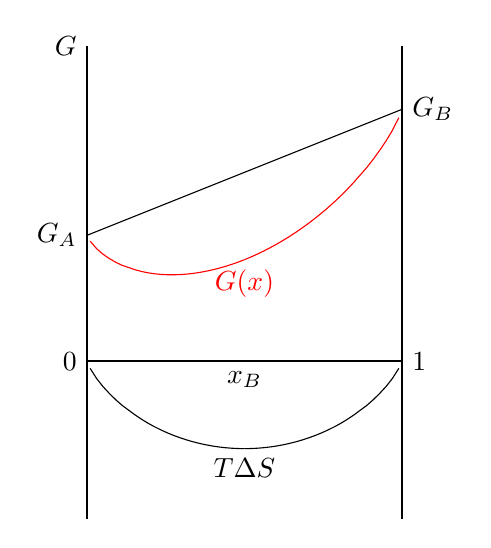
\begin{tikzpicture}[scale=4]
            \draw[thick] (0,0) node[anchor=east]{0} --(0.5,0) node[anchor=north] {$x_B$}--(1,0) node[anchor=west]{1};
            \draw[thick] (0,-0.5) -- (0,0.4) node[anchor=east]{$G_A$}--(0,1) node[anchor=east]{$G$};
            \draw[thick] (1,-0.5) -- (1,0.8) node[anchor=west]{$G_B$}--(1,1);
            
            \draw[thin] (0,0.4)--(1,0.8);
            \draw[domain=0.01:0.5] plot(\x,{0.4*(\x*ln(\x)+(1-\x)*ln((1-\x)))})
                node[below] {$T\Delta S$};
            \draw[domain=0.5:0.99] plot(\x,{0.4*(\x*ln(\x)+(1-\x)*ln((1-\x)))});
            %G(x)
            \draw[red,domain=0.01:0.5] plot(\x,{0.4*\x+0.4+0.4*(\x*ln(\x)+(1-\x)*ln((1-\x)))})
                node[below] {$G(x)$};
            \draw[red,domain=0.5:0.99] plot(\x,{0.4*\x+0.4+0.4*(\x*ln(\x)+(1-\x)*ln((1-\x)))});        
        \end{tikzpicture}
       % \caption{$\Delta H^M=0$,混合时结合能不变的自由能曲线。}
        \label{混合时结合能不变的自由能曲线}
    }
   % \end{subfigure}
   % \begin{subfigure}[0.3\textwidth]
    \subfigure[混合时结合能减小的自由能曲线]
    {
           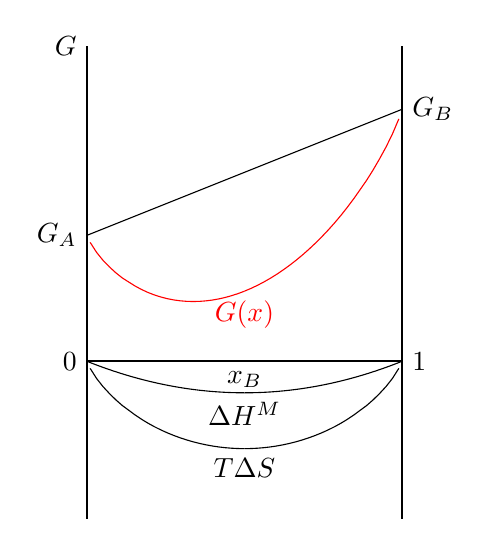
\begin{tikzpicture}[scale=4]
            \draw[thick] (0,0) node[anchor=east]{0} --(0.5,0) node[anchor=north] {$x_B$}--(1,0) node[anchor=west]{1};
            \draw[thick] (0,-0.5) -- (0,0.4) node[anchor=east]{$G_A$}--(0,1) node[anchor=east]{$G$};
            \draw[thick] (1,-0.5) -- (1,0.8) node[anchor=west]{$G_B$}--(1,1);
            %G(0)
            \draw[thin] (0,0.4)--(1,0.8);
            %T\Delta S
            \draw[domain=0.01:0.5] plot(\x,{0.4*(\x*ln(\x)+(1-\x)*ln((1-\x)))})
                node[below] {$T\Delta S$};
            \draw[domain=0.5:0.99] plot(\x,{0.4*(\x*ln(\x)+(1-\x)*ln((1-\x)))});
            %\Delta H
            \draw[domain=0:0.5] plot(\x,{-0.4*(\x*(1-\x))})
                node[below] {$\Delta H^M$};
            \draw[domain=0.5:1] plot(\x,{-0.4*(\x*(1-\x))});
            
            %G(x)
            \draw[red,domain=0.01:0.5] plot(\x,{0.4*\x+0.4-0.4*(\x*(1-\x))+0.4*(\x*ln(\x)+(1-\x)*ln((1-\x)))})
                node[below] {$G(x)$};
            \draw[red,domain=0.5:0.99] plot(\x,{0.4*\x+0.4-0.4*(\x*(1-\x))+0.4*(\x*ln(\x)+(1-\x)*ln((1-\x)))});        
        \end{tikzpicture}
        %\caption{$\Delta H^M<0$,混合时结合能小于零的自由能曲线。}
        \label{混合时结合能减小的自由能曲线}
    }
    
    %\end{subfigure}
    \caption{三种不同情况的自由能曲线}
\end{figure}


                当焓变小于零时,也就是$\Delta H^M<0$,
                \begin{equation}
                    \frac{\partial^{2} G}{\partial x_{B}^{2}}=2 \alpha^{\prime}+R T\left(\frac{1}{x_{A}}+\frac{1}{x_{B}}\right)<0,
                \end{equation}
                这时异类原子的结合力大于同类原子之间的结合力。表现为在溶解时会放出热量。此时$G(x)$为下垂线,曲线的凹陷更大,如\autoref{混合时结合能减小的自由能曲线}所示。

                当焓变大于零时,焓变与熵的变化为相反的作用,曲线的形状与两者的大小有关。
                
                
                \begin{figure}[ht]
    \centering
    %\begin{subfigure}[0.3\textwidth]
    \subfigure[$T>\frac{\alpha^{\prime}}{2R}$]
    {
        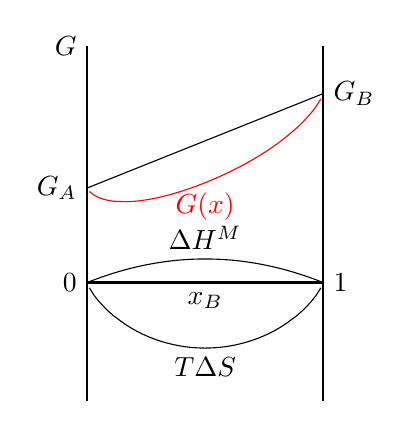
\begin{tikzpicture}[scale=3]
            \draw[thick] (0,0) node[anchor=east]{0} --(0.5,0) node[anchor=north] {$x_B$}--(1,0) node[anchor=west]{1};
            \draw[thick] (0,-0.5) -- (0,0.4) node[anchor=east]{$G_A$}--(0,1) node[anchor=east]{$G$};
            \draw[thick] (1,-0.5) -- (1,0.8) node[anchor=west]{$G_B$}--(1,1);
            
            \draw[thin] (0,0.4)--(1,0.8);
            \draw[domain=0.01:0.5] plot(\x,{0.4*(\x*ln(\x)+(1-\x)*ln((1-\x)))})
                node[below] {$T\Delta S$};
            \draw[domain=0.5:0.99] plot(\x,{0.4*(\x*ln(\x)+(1-\x)*ln((1-\x)))});
            
            %\Delta H
            \draw[domain=0:0.5] plot(\x,{0.4*(\x*(1-\x))})
                node[anchor=south] {$\Delta H^M$};
            \draw[domain=0.5:1] plot(\x,{0.4*(\x*(1-\x))});
            
            %G(x)
            \draw[red,domain=0.01:0.5] plot(\x,{0.4*\x+0.4+0.4*(\x*(1-\x))+0.4*(\x*ln(\x)+(1-\x)*ln((1-\x)))})
                node[below] {$G(x)$};
            \draw[red,domain=0.5:0.99] plot(\x,{0.4*\x+0.4+0.4*(\x*(1-\x))+0.4*(\x*ln(\x)+(1-\x)*ln((1-\x)))});        
        \end{tikzpicture}
       % \caption{$\Delta H^M=0$,混合时结合能不变的自由能曲线。}
        \label{subfig:高温下混合时结合能增加的自由能曲线}
    }
   % \end{subfigure}
   % \begin{subfigure}[0.3\textwidth]
    \subfigure[$0<T<\frac{\alpha^{\prime}}{2R}$]
    {
           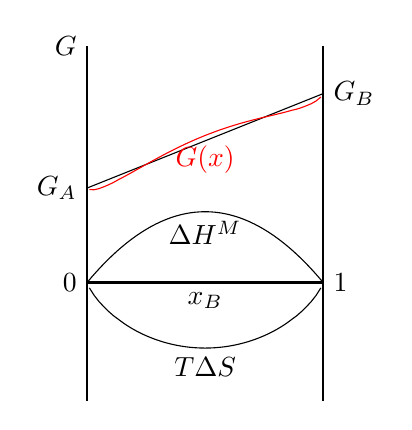
\begin{tikzpicture}[scale=3]
            \draw[thick] (0,0) node[anchor=east]{0} --(0.5,0) node[anchor=north] {$x_B$}--(1,0) node[anchor=west]{1};
            \draw[thick] (0,-0.5) -- (0,0.4) node[anchor=east]{$G_A$}--(0,1) node[anchor=east]{$G$};
            \draw[thick] (1,-0.5) -- (1,0.8) node[anchor=west]{$G_B$}--(1,1);
            %G(0)
            \draw[thin] (0,0.4)--(1,0.8);
            %T\Delta S
            \draw[domain=0.01:0.5] plot(\x,{0.4*(\x*ln(\x)+(1-\x)*ln((1-\x)))})
                node[below] {$T\Delta S$};
            \draw[domain=0.5:0.99] plot(\x,{0.4*(\x*ln(\x)+(1-\x)*ln((1-\x)))});
            %\Delta H
            \draw[domain=0:0.5] plot(\x,{1.2*(\x*(1-\x))})
                node[below] {$\Delta H^M$};
            \draw[domain=0.5:1] plot(\x,{1.2*(\x*(1-\x))});
            
            %G(x)
            \draw[red,domain=0.01:0.5] plot(\x,{0.4*\x+0.4+1.2*(\x*(1-\x))+0.4*(\x*ln(\x)+(1-\x)*ln((1-\x)))})
                node[below] {$G(x)$};
            \draw[red,domain=0.5:0.99] plot(\x,{0.4*\x+0.4+1.2*(\x*(1-\x))+0.4*(\x*ln(\x)+(1-\x)*ln((1-\x)))});        
        \end{tikzpicture}
        %\caption{$\Delta H^M<0$,混合时结合能小于零的自由能曲线。}
        \label{subfig:低温下混合时结合能增加的自由能曲线}
    }
    \subfigure[$T=0$]
    {
        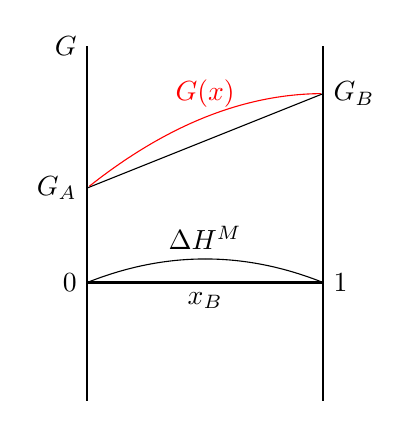
\begin{tikzpicture}[scale=3]
            \draw[thick] (0,0) node[anchor=east]{0} --(0.5,0) node[anchor=north] {$x_B$}--(1,0) node[anchor=west]{1};
            \draw[thick] (0,-0.5) -- (0,0.4) node[anchor=east]{$G_A$}--(0,1) node[anchor=east]{$G$};
            \draw[thick] (1,-0.5) -- (1,0.8) node[anchor=west]{$G_B$}--(1,1);
            %G(0)
            \draw[thin] (0,0.4)--(1,0.8);
            %T\Delta S
            %\draw[domain=0.01:0.5] plot(\x,{0.4*(\x*ln(\x)+(1-\x)*ln((1-\x)))})
            %    node[below] {$T\Delta S$};
            %\draw[domain=0.5:0.99] plot(\x,{0.4*(\x*ln(\x)+(1-\x)*ln((1-\x)))});
            %\Delta H
            \draw[domain=0:0.5] plot(\x,{0.4*(\x*(1-\x))})
                node[anchor=south] {$\Delta H^M$};
            \draw[domain=0.5:1] plot(\x,{0.4*(\x*(1-\x))});
            
            %G(x)
            \draw[red,domain=0.01:0.5] plot(\x,{0.4*\x+0.4+0.4*(\x*(1-\x))})
                node[anchor=south] {$G(x)$};
            \draw[red,domain=0.5:0.99] plot(\x,{0.4*\x+0.4+0.4*(\x*(1-\x))});        
        \end{tikzpicture}
        %\caption{$\Delta H^M<0$,混合时结合能小于零的自由能曲线。}
        \label{subfig:绝对零度下混合时结合能增加的自由能曲线}
    }
    %\end{subfigure}
    \caption{混合时结合能增加的在不同温度下的自由能曲线}

\end{figure}

                
                当$T\geq\frac{\alpha^{\prime}}{2R}$时,混合所提高的内能全部由热温熵来补充,$\Delta G^m\leq0$,曲线仍然为下垂曲线,仅仅是下垂的程度小一点,如\autoref{subfig:高温下混合时结合能增加的自由能曲线}所示。

                在低温情况下,$T<\frac{\alpha^{\prime}}{2R}$时,构成的曲线有三个极值点和两个拐点,在靠近坐标轴($x$接近0或1)处为上凹曲线,有两个极小值,而中部位凹向朝下的上凸曲线,会有一极大值,如\autoref{subfig:低温下混合时结合能增加的自由能曲线}所示。
                在这种情况下,存在两种必然的规律:
                \begin{enumerate}
                    \item[1] 任何一个组元都可以少量溶解其它组元,不可能得到绝对的纯净物质;
                    \item[2] 当出现上凸时,吉布斯自由能会提高,自发的趋势是形成两相混合物可以降低体系的自由能,两组元表现为有限溶解。
                \end{enumerate}
    \section{均匀形核}
        相变动力学\index{相变动力学}是讨论相变的过程和速度的,新相的形核\index{形核}和长大\index{长大}是动力学的两个基本问题。

        即使在宏观的单相均匀系统中,也存在着微观的不均匀性,存在局部的能量、密度、成分组态的涨落。Gibbs将这种涨落分为两类:
        \begin{enumerate}
            \item[1] 在\textbf{很小的体积}内存在着剧烈的原子再分布,在亚稳的母相中形成\textbf{新相胚芽},当这种胚芽超过临界尺寸\index{形核!临界尺寸},就变成稳定的新相核心而自发长大,金属和合金中的转变多数如此;
            \item[2] 在\textbf{大的体积内}原子的少量调整,\textbf{转变在整个体积范围内进行},如有序-无序转变\index{有序-无序转变}。
        \end{enumerate}

        以纯金属的凝固为例,假设在$L$中形成半径为$r$的晶核\index{形核!晶核}$s$,固体和液体的体积为$V_s$和$V_L$,固体和液体单位体积的自由能为$G_v^s$、$G_v^L$,$A_{SL}$为两相之间面积,$r_{SL}$为两相的界面能。

        假设发生相变的过程中没有体积变化,没有形核时,体系的自由能为
        \begin{equation}
            G_1=\left( V_s+V_l \right)G_v^L,
        \end{equation}
        则体系中出现晶核的自由能为:
        \begin{equation}
            G_2=V_sG_v^S+V_LG_v^L+A_{SL}\gamma_{SL},
        \end{equation}
        所以形核时的自由能变化为
        \begin{equation}
            \Delta G_v=G_2-G_1=-V_S\cdot \Delta G_v++A_{SL}\gamma_{SL},
        \end{equation}
        式中$\Delta G_v=G_v^L-G_v^S$。
        
        假设晶核为球形,则固液界面面积和固体体积为
        \begin{equation}
            A_{SL}=4\pi r^2, V=\frac{4}{3}\pi r^3,
        \end{equation}
        形核的自由能变化量为
        \begin{equation}
            \Delta G_r=-\frac{4}{3}\pi r^3\Delta G_v+4\pi r^2\gamma_{SL},
        \end{equation}
        在平衡状态下,对$r$求导,
        \begin{equation}
            \frac{\dif \Delta G_r }{\dif r}=-4\pi r^2\Delta G_v+8\pi r\gamma_{SL},
        \end{equation}
        令导数为零,此时的晶核半径为临界晶核尺寸\index{临界晶核尺寸}
        \begin{equation}
            r^*=\frac{\gamma_{SL}}{\Delta G_v}.
        \end{equation}
        自由能改变量为
        \begin{equation}
            \Delta G^*=\frac{16\pi}{3}\left( \frac{\gamma_{SL}^3}{\Delta G_v^2} \right),
        \end{equation}
        根据自由能的二阶导数可知,此时的自由能为极大值。因此只有半径大于临界晶核尺寸的晶核才能继续长大,而小于该尺寸的晶核则消失。
        临界晶核对于的自由能变化量$\Delta G^*$为形核功,即核长大到$r^*$所需克服的势垒。

        形核功的量值是临界球形晶核表面能的$1/3$,也就是说,球形晶核的表面能的$2/3$由新相的自由能下降给出,
        $1/3$依靠热涨落。这一过程称为\textbf{热激活过程}\index{形核!热激活过程}。

        在凝固过程中,要达到临界半径,需要温度上提供足够的过冷度,假设熔点温度为$T_m$,外界温度与熔点温度差为$\Delta T$,
        此时的自由能变化量为
        \begin{equation}
            \Delta G_v=\frac{\Delta T\cdot\Delta H_m}{T_m},
        \end{equation}
        代入临界半径表达式为
        \begin{equation}
            r^*=\frac{2\gamma_{LS}T_m}{\Delta H_m\cdot\Delta T},
        \end{equation}
        因此当$\Delta T=0$,$\Delta G^*\to0$,不能形核,过冷度越大,越易形核。
    \section{形核速率及均匀形核在固态转变中的推广}
        在液态的情况下,金属中也会存在一些小区域具有固态的密堆结构,本章将对这些小区域进行讨论。

        假设在单位体积内,由$i$个分子组成半径为$r$的胚芽数为$n_i$,而单分子数目为$n$,
        而单位体积中独立质点数$N$为
        \begin{equation}
            N=n+\sum_{i\geq2}n_i,
        \end{equation}
        由于$\sum_{i\geq2}n_i\ll n$,所以$N$约等于单位体积中的分子数。从统计方面考虑,胚芽数$n_i$服从玻尔兹曼分布:
        \begin{equation}
            n_i=N e^{-\frac{\Delta G_r}{kT}},
        \end{equation}
        临界核心数$n_i^*$为
        \begin{equation}
            n_i^*=N e^{-\frac{\Delta G_r^*}{kT}},
        \end{equation}
        其中$\Delta G_r^*$为形核功。

        在临界核心上痛殴分子碰撞再增加一个分子,它就可以克服势垒称为稳定的新相核心。
        定义单位体积中单位时间内形成的新相稳定核心的数目为形核速率\index{形核速率}$I$,
        所以形核速率$I$正比于临近核心的分子加入核心的频率$\omega$,即
        \begin{equation}
            I=\omega\cdot n_i^*=\omega N e^{-\frac{\Delta G_r^*}{kT}}\label{形核速率},
        \end{equation}
        $\omega$取决于原子振动频率、扩散激活能、晶核的表面积等。

        \subsection{形核引起的晶格畸变}
            在金属相变的过程中,由于晶核周围的体积和形状可能发生变
            化,或者晶核受到周围晶格的限制,使得晶核中的原子不能处
            在平衡位置,这两种情况都消耗弹性应变能$\varepsilon$,这种弹性应变
            能通过扩散和范性流变才能松弛。

            假定应变能正比于晶核的体积,则形核的自由能写作
            \begin{equation}
                \Delta G_r=-\frac{4}{3}\pi \cdot r^3(\Delta G_v+\varepsilon)+4\pi\cdot r^2\cdot\gamma_{SL},
            \end{equation}
            临界半径变为
            \begin{equation}
                r^*=\frac{2\gamma_{SL}}{\Delta G_v+\varepsilon},
            \end{equation}
            形核功为
            \begin{equation}
                \Delta G^*=\frac{16\pi \gamma^3_{SL}}{3(\Delta G_v+\varepsilon)^2}.
            \end{equation}
            另外,假设晶核的表面积对此时的邻近核心的分子加入核心的频率$\omega$没有影响,可以写为
            \begin{equation}
                \omega=ve^{-\frac{\Delta G_m}{kT}},
            \end{equation}
            其中$v$是原子振动频率\index{形核速率!原子振动频率},$\Delta G_m$是原子扩散的激活能\index{形核速率!扩散激活能}。所以\autoref{形核速率}可以写为
            \begin{equation}
                I=Nve^{-\frac{\Delta G^*+\Delta G_m}{kT}}\label{考虑外来扩散原子的形核速率},
            \end{equation}
            式中,$Nv$对$I$的影响很小,形核速率强烈依赖指数因子,也就是形核功和原子扩散激活能。
            对于固态相变,合理的数量级为
            \begin{equation*}
                Nve^{-\frac{\Delta G_m}{kT}}\simeq 10^{30},I=10^{30}e^{-\frac{\Delta G^*}{kT}}.
            \end{equation*}

            由于$\Delta G^*$因过冷度$\Delta T$的增大而减小,所以\textbf{形核速率强烈依赖于温度}。
            当$\Delta T\to0$,$\Delta G^*\to\infty$,$I\to0$,$\Delta T$增大,形核速率$I$存在极值,
            先增大后减小。

            \begin{figure}[ht]
                \centering
                    \subfigure[某合金的局部相图。]
                    {
                        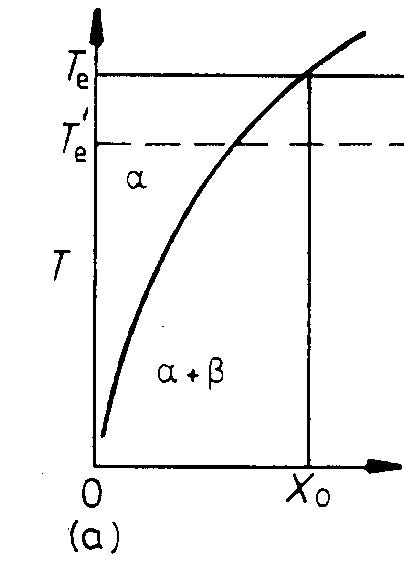
\includegraphics{fig/均匀形核速率I与转变温度之间的关系/a.jpg}
                        \label{subfigure:某合金的局部相图}
                    }
                    \subfigure[相图的有效推动能量与形核功与转变温度之间的关系。]
                    {
                        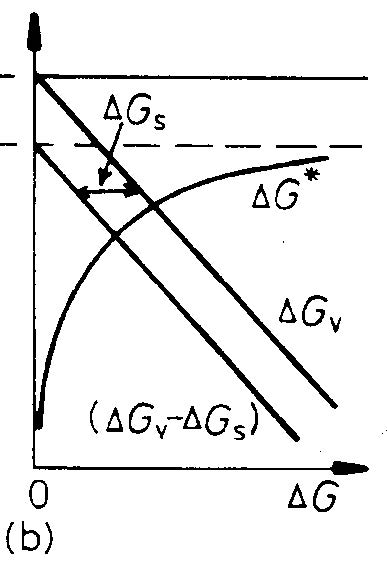
\includegraphics{fig/均匀形核速率I与转变温度之间的关系/b.jpg}
                    }
                    \\
                    \subfigure[确定$I$的两个指数项与温度的关系。]
                    {
                        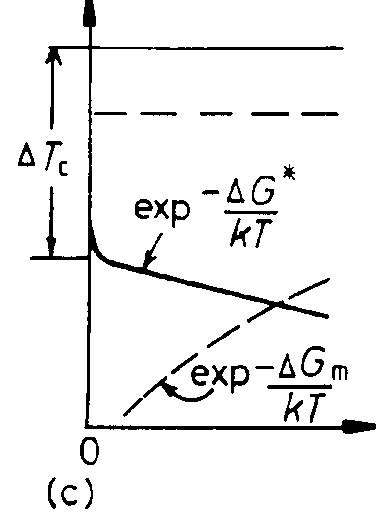
\includegraphics{fig/均匀形核速率I与转变温度之间的关系/c.jpg}
                    }
                    \subfigure[$I $随温度的变化。]
                    {
                        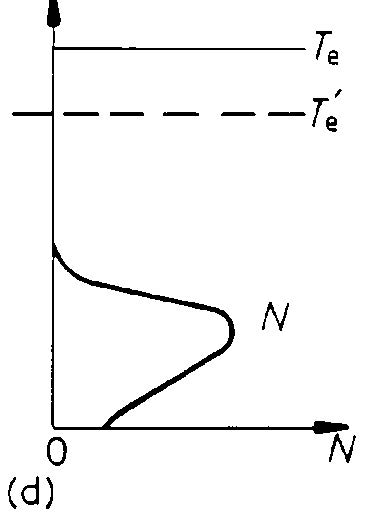
\includegraphics{fig/均匀形核速率I与转变温度之间的关系/d.jpg}
                        \label{subfigure:$I $随温度的变化}
                    }
                \caption{均匀形核速率$I$与转变温度之间的关系。}
                \label{均匀形核速率I与转变温度之间的关系}
            \end{figure}

            从\autoref{subfigure:某合金的局部相图}可知,成分为$x_0$的合金,其固溶温度为$T_e$,为了抵消应变能$\Delta G_\varepsilon$,
            必须过冷到$T_e^{\prime}$才能析出第二相$\beta$。形核速率随$T$的变化如\autoref{subfigure:$I $随温度的变化}所示,
            在高温下,沉淀的推动能量很小,因为$\Delta G^*$很大,所以$I$很小;在低温情况下,由于扩散很慢,所以$I$也很小,在中间某一个温度,
            $I$有极大值。

        \subsection{相界面性质的影响}

            界面能\index{界面能}$\gamma$的来源可以分为两部分,
            \begin{itemize}
                \item[1] 一部分是在母相中形成新相界面时,同类键和异类键的数量变化引起的,称为界面能中的\textbf{化学项}\index{界面能!化学项};
                \item[2] 另一部分是界面结构引起的 (如界面上产生的位错),称为界面能中的\textbf{结构项}\index{界面能!结构项}。
            \end{itemize}
            
            如果新相和母相的晶体结构和取向相同,电阵常数也非常接近,形成\textbf{完全共格界面}\index{完全共格界面}。界面能
            较小,只包括化学项,结构项(畸变能$\varepsilon$)趋于0,长大速度很快。

            如果完全共格两相的点阵常数不同,就会在界面上引入位错,来减少界面能中的体积应变能,结构项略有增大,形成\textbf{部分共格界面}\index{部分共格界面}。

            若新相通过母相切变形成,某些界面点阵相似,这种界面称为\textbf{切变共格}\index{切变共格}。

            如果所有界面都不共格,称为\textbf{非共格}\index{非共格}新相。

            
    \section{非均匀形核(界面形核)}
        
    \section{过饱和固溶体的脱溶沉淀}
    \section{调幅分解}
    \section{马氏体相变}